\documentclass{article}

\usepackage[english]{babel}
\usepackage[a4paper,top=2cm,bottom=2cm,left=3cm,right=3cm,marginparwidth=1.75cm]{geometry}

\usepackage{amsmath}
\usepackage{graphicx}
\usepackage{minted}

\usepackage[colorlinks=true, allcolors=blue]{hyperref}

\title{Solving 2048 with Expectimax}
\author{David Cook}

\begin{document}
\maketitle

\tableofcontents

\begin{abstract}
The simplest goal of this project is to play the puzzle game 2048 with the expectimax algorithm. I intend to make it able to play any size of 2048 game, though eventually, any algorithm will break down if the grid is too large. In order to mitigate this, I intend to find ways of pruning the tree as much as possible. 
\end{abstract}
\section{Introduction}
\label{sec:intro}
\section{Proof of Concepts}
\label{sec:proof_of_concepts}
\subsection{Decision Tree}
\label{subsec:dt}
There are many ways of implementing a tree structure, various ones are more appropriate than others. The operations that a required in this situation are \cite{russell2010artificial}:
\begin{itemize}
    \item Generate a tree from the root node.
    \item Transverse the entire tree to calculate the score.
    \item Walk to a direct child node and regenerate the tree. At least the scores will need to regenerate on pre-existing nodes.
\end{itemize}
While this will likely not be true, I will assume generating a node can be done in $O(1)$ time. Generating or traversing nodes in a tree, with $n$ nodes, can not be done in any less than $O(n)$. Reading a direct child can not be done in $O(1)$ time. \par
A common approach to making a tree is as follows:
\begin{minted}{java}
public class Node {
    int value;
    Node[] children;
}
\end{minted}
This is a node with an array of references to its child nodes. Traversing this entire tree will have a time complexity of $O(n)$. Arranging these nodes into a tree structure takes $O(n)$ and finally picking a direct child of a node takes $O(1)$, Therefore there is no need to pick a less common tree implementation.

\subsection{Expectimax}
\label{subsec:expectimax}
\begin{figure}
    \centering
    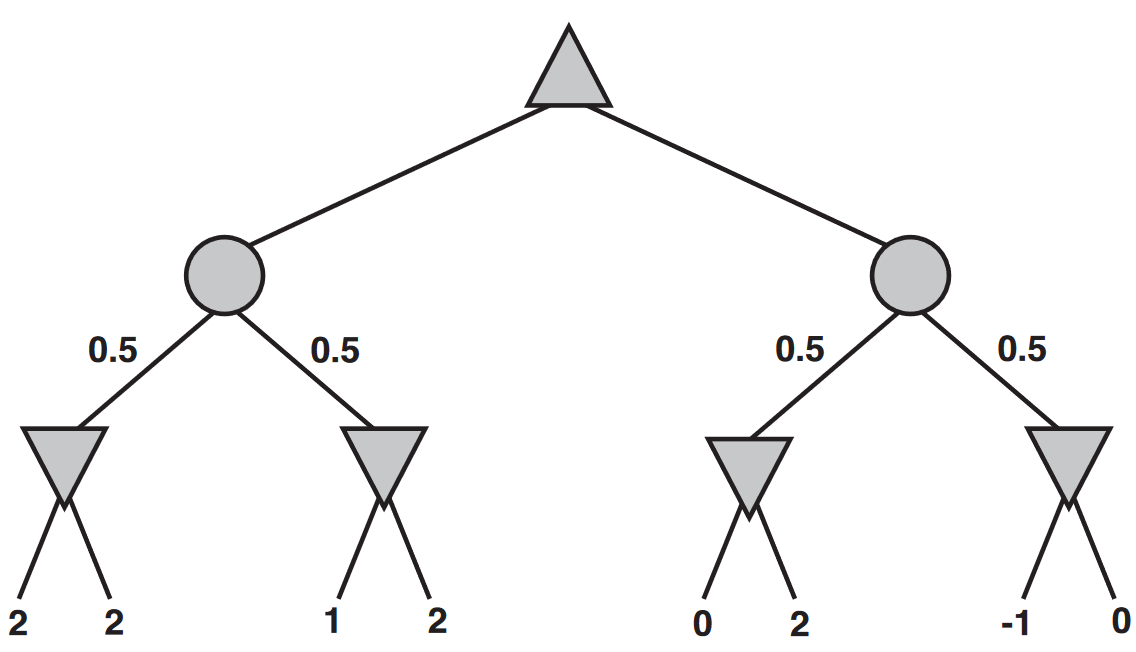
\includegraphics[width=0.7\textwidth]{expectimax.png}
    \caption{An image of an expectimax tree \cite[p.~200]{russell2010artificial}}
    \label{fig:expectree}
\end{figure}
The decision tree required in the expectimax algorithm (Figure \ref{fig:expectree}) has three types of nodes, however, only two types of nodes are needed for the problem of solving 2048. These three types of nodes include:
\begin{itemize}
    \item Maximizing nodes: These nodes get the maximum scoring child of the node, and acquire the same score
    \item Chance Nodes: These nodes represent situations where there are random states that may follow. The weights of the link between a chance node and its children represent the probabilities of that event occurring.
    \item Minimizing Nodes: These are the opposite of maximizing nodes, I do not expect to need them in this project.
    \item Terminus nodes: These nodes are the leaves of the tree. Their score is already known and used to calculate the score in the rest of the tree.
\end{itemize}
Each of these three relevant types nodes have been converted to individual java classes, storing the scores in a float attribute. This means that the value of the score only needs to be retrieved once.

\subsection{2048}
\subsection{2048 with Expectimax}
\subsection{Heuristic for 2048}

\section{2048 Game}
\section{Design Patterns for AI Search}
\section{Techniques used to solve the game}
\subsection{Human Approaches}
\subsection{Automated Approaches}
\section{User Interface Design}
\section{Complexity}
\subsection{Time Complexity}
\subsection{NP Hardness}

\bibliographystyle{plain}
\bibliography{Artificial_Intelligence}

\end{document}